\documentclass[preprint,11pt]{elsarticle}
\usepackage[margin=2.5cm]{geometry}

\usepackage{graphicx} 
\usepackage{hyperref} 
\usepackage{mathtools}
\usepackage{amsmath}    
\usepackage{amssymb} 

\title{Fully Dynamic \textit{k}-Center Clustering in Low Dimensional Metrics}

\author[toronto]{Gramoz Goranci\corref{cor1}}
\author[vienna]{Monika Henzinger}
\author[vienna]{Dariusz Leniowski}
\author[heidelberg]{Christian Schulz}
\author[vienna]{Alexander Svozil}

% \cortext[cor1]{Corresponding author.}

\address[toronto]{Department of Computer Science, University of Toronto, Canada.}
\address[vienna]{Theory and Application of Algorithms, University of Vienna, Austria.}
\address[heidelberg]{Faculty of Mathematics and Computer Science, Heidelberg University, Germany.}

\fntext[funding]{The research leading to these results has received funding from the European Research Council under the European Union's Seventh Framework Programme (FP/2007–2013) / ERC Grant Agreement no. 340506, and from the Vienna Science and Technology Fund (WWTF) through project ICT15–003.}

\begin{document}


\begin{abstract}

Clustering is one of the most fundamental problems in unsupervised learning with a large number of applications. However, classical clustering algorithms assume that the data is static, thus failing to capture many real-world applications where data is constantly changing and evolving. Driven by this, we study the metric $k$-center clustering problem in the fully dynamic setting, where the goal is to efficiently maintain a clustering while supporting an intermixed sequence of insertions and deletions of points. This model also supports queries of the form (1) report whether a given point is a center or (2) determine the cluster a point is assigned to. We present a deterministic dynamic algorithm for the $k$-center clustering problem that provably achieves a (2 +$\epsilon$)-approximation in nearly logarithmic update and query time, if the underlying metric has bounded doubling dimension, its aspect ratio is bounded by a polynomial and $\epsilon$ is a constant. An important feature of our algorithm is that the update and query times are independent of $k$. We confirm the practical relevance of this feature via an extensive experimental study which shows that for large values of $k$, our algorithmic construction outperforms the state-of-the-art algorithm in terms of solution quality and running time.
\end{abstract}

\maketitle
\section{Introduction}

The $k$-center clustering problem is a crucial optimization task in computational geometry and machine learning, commonly used in applications like facility location, data compression, and social network analysis. It involves selecting $k$ center points to minimize the maximum distance between any data point and its nearest center. In real-world scenarios, where data is dynamic and constantly evolving, traditional static clustering methods fall short. To address this, we propose a fully dynamic algorithm for $k$-center clustering that adapts to data insertions, deletions, and queries in real-time, maintaining a high-quality solution. Our approach leverages navigating nets, offering a $(2 + \varepsilon)$-approximation factor, while ensuring performance independent of $k$. Through extensive evaluations, we demonstrate significant improvements in both solution quality and speed over existing state-of-the-art algorithms.


\section{Preliminaries}
In the \textit{k}-center clustering problem, we are given a set $\mathit{M}$ of points equipped with some metric $d$ and an integer parameter $k > 0$. The goal is to find a set $C = \{ c_1, \dots, c_k \}$ of $k$ points (centers) so as to minimize the quantity $\phi(C) = \max_{x \in M} d(x, C)$, where $d(x, C) = \min_{c \in C} d(x, c)$. Let OPT denote the cost of the optimal solution.

In the \textit{dynamic} version of this problem, the set $M$ evolves over time and queries can be asked. Concretely, at each timestep $t$, either a new point is added to $M$, removed from $M$, or one of the following queries is made for any given point $x \in M$: 
(i) decide whether $x$ is a center in the current solution, and 
(ii) find the center $c$ to which $x$ is assigned. The goal is to maintain the set of centers $C$ after each client update so as to maintain a small factor approximation to the optimal solution.

Let $d_{\text{min}}$ and $d_{\text{max}}$ be lower and upper bounds on the minimum and maximum distance between any two points that are ever inserted. For each $x \in M$ and radius $r$, let $B(x, r)$ be the set of all points in $M$ that are within distance $r$ from $x$, i.e., $B(x, r) := \{ y \in M \mid d(x, y) \leq r \}$.

\section{Fully dynamic \textit{k}-center clustering using navigating nets}


In this section, we present a fully-dynamic algorithm for the \textit{k}-center clustering problem that achieves a $(2 + \varepsilon)$-approximation with a running time not depending on the number of clusters $k$. The first component of our algorithm is to use a nearest neighbor search data structure called “navigating nets” (Krauthgamer and Lee \cite{krauthgamer2004navigating}). Unfortunately, this technique by itself only guarantees an 8-approximation, which does not suffice to obtain the claimed $(2 + \varepsilon)$-approximation factor. The second part of our construction is a seemingly unrelated scaling argument by McCutchen and Khuller \cite{mccutchen2008streaming} used in the context of incremental streaming algorithms. Our work is the first to apply this argument together with the nearest neighbor search data structures.

We start by reviewing notation from \cite{krauthgamer2004navigating}. 

\textit{r-\textbf{\text{net}}}. Let $(X, d)$ be a metric space. For a given parameter $r > 0$, a subset $Y_r \subseteq X$ is an \textit{r-net} of $X$ if the following properties hold:

\begin{enumerate}
    \item (separating) Distinct $x, y \in Y_r$ have $d(x, y) \geq r$.
    \item (covering) $X \subseteq \bigcup_{y \in Y_r} B(y, r)$.
\end{enumerate}

    \subsection{Navigating Nets}  
    Given a metric space $(M, d)$ which evolves over time with parameters $d_{\text{min}}$ and $d_{\text{max}}$, we define $\Gamma := \{\alpha^i : i \in \mathbb{Z}\}$ as the set of scales of $(M, d)$ for some $\alpha > 1$. We define an \textit{r}-net for all $r \in \Gamma$ as follows: For all $r < d_{\text{min}}$, we define $Y_r := M$ as a trivial $r$-net of $M$. For $r > d_{\text{min}}$, define $Y_r$ to be an $r$-net of $Y_{r/\alpha}$. Note that $Y_r$ is a subset of $Y_{r/\alpha}$ and contains a point with distance $\leq r$ to every point in $Y_{r/\alpha}$. 
    
    A navigating net $\Pi$ is defined as the union over all $Y_r$ for $r \in \Gamma$. We refer to the elements in $Y_r$ as centers. Note that for every scale $r > d_{\text{max}}$, the set $Y_r$ contains only one element due to the separating property. A navigating net $\Pi$ keeps track of (i) the smallest scale $r_{\text{max}}$ defined by $r_{\text{max}} = \min\{r \in \Gamma : \forall r' \geq r, |Y_{r'}| = 1\}$, and (ii) the largest scale $r_{\text{min}}$ defined by $r_{\text{min}} = \max\{r \in \Gamma : r' \leq r, Y_{r'} = M\}$. All scales $r \in \Gamma$ such that $r \in [r_{\text{min}}, r_{\text{max}}]$ are referred to as nontrivial scales. Figure \ref{fig:navigating_net_example} illustrates an example of a navigating net.


    \begin{figure}[h]
    \centering
    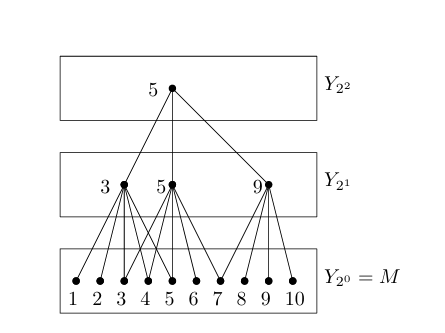
\includegraphics[width=0.5\linewidth]{graph.png} % Replace with the actual image file   
    \caption{An example for a navigating net with $M = \{1, 2, 3, 4, 5, 6, 7, 8, 9, 10\}$ where $d$ is Euclidean and $\alpha = 2$. Consequently, $\Gamma = \{2^i : i \in \mathbb{Z}\}$. In the navigating net, the nontrivial scales are given by $\{2^0, 2^1, 2^2\}$. Consequently, $r_{\text{max}} = 2^2$, $r_{\text{min}} = 2^0$.}
    \label{fig:navigating_net_example}
    \end{figure}





\section{Empirical Analysis}
In this section, we present the experimental evaluation for our \textit{k}-center algorithm. We implemented the algorithm described in the previous sections using cover trees \cite{beygelzimer2006cover, kollar2006fast}, which is a fast variant of navigating nets. The cover tree maintains the same invariants as navigating nets, except that for a point at a certain level in the hierarchy, we store \textit{exactly one} nearby point one level up, instead of a set of points that are nearby. Beygelzimer et al. \cite{beygelzimer2006cover} show that all running time guarantees can be maintained for metric spaces with bounded expansion constant. This in turn implies that using a collection of cover trees yields a $(2 + \varepsilon)$-approximation for the \textit{k}-center clustering problem. The expansion constant of $M$ is defined as the smallest value $c \geq 2$ such that $\left| B(p, 2r) \right| \leq c \left| B(p, r) \right|$ for all $p \in M$ and $r > 0$. Our algorithm maintains $O(\varepsilon^{-1} \ln \varepsilon^{-1})$ cover trees. To obtain the current centers of a cover tree, we traverse the tree top-down and add all distinct points until we have $k$ points. Due to the \textit{nesting property} of the cover tree, i.e., every point which appears in some level $i$ appears in every lower level $j < i$ in the tree \cite{beygelzimer2006cover}, we are guaranteed to add all nodes of the desired level $Y^p_r$ described in Section 3.2. From now on we call our algorithm $A_{\text{Cov}}$. 

We compare our algorithm against the algorithm of Chan et al. \cite{hubert2018dynamic} which is the state-of-the-art approach for the fully dynamic \textit{k}-center problem in practice.


\subsection{The algorithm of Chan et al. \cite{hubert2018dynamic}}
To gain some intuition into the state-of-the-art algorithm in practice, we give a brief summary of the algorithm described in Chan et al. \cite{hubert2018dynamic}: The algorithm maintains a clustering for each $r \in \Gamma := \{(1 + \varepsilon)^i : d_{\text{min}} \leq (1 + \varepsilon)^i \leq d_{\text{max}}, i \in \mathbb{N}\}$. Their algorithm is a $(2 + \varepsilon)$-approximation of the optimal solution and has an average running time of $O(k^2 \cdot \frac{\log(\Delta)}{\varepsilon})$ per update. 

Note that the algorithm needs $d_{\text{min}}$ and $d_{\text{max}}$ as input and that it is not guaranteed that these values are available in practice. In contrast, $A_{\text{Cov}}$ does not need these parameters. For our empirical analysis, we provided these special parameters to the algorithm of Chan et al. \cite{hubert2018dynamic}. For arbitrary instances, one would initialize $d_{\text{min}}, d_{\text{max}}$ with the minimum/maximum value for the type `double` respectively to guarantee the correctness of their algorithm. From now on, we call their algorithm $A_{\text{CGS}}$.
 \subsection{Setup}
    We implemented the cover tree in C++ and compiled it with g++-7.4.0. We executed all of our experiments on a Linux machine running on an AMD Opteron Processor 6174 with 2.2GHz and 256GB of RAM. In our experiments, we evaluate $A_{\text{CGS}}$ and $A_{\text{Cov}}$ with the following pairwise combinations of $\varepsilon \in \{0.1, 0.5, 1, 4\}$ and $k \in \{20, 50, 100, 200\}$. In total, we perform 10 different runs for each test instance and compute the arithmetic mean of the solution improvement and speedup on this instance. When further averaging over multiple instances, we use the geometric mean in order to give every instance a comparable influence on the final score. To measure the solution quality of an algorithm at any timepoint $i$ we query for the current set of centers $C_i$. We do not directly compute the objective function value $\phi(C_i)$, since this is an expensive operation and it is not usually needed in practice. After the termination of the two algorithms, we compute the objective function of the \textit{k}-center solution $\phi(C_i)$ in order to compare the solutions of the two competing algorithms $A_{\text{Cov}}$ and $A_{\text{CGS}}$. Hence, the running times of both algorithms include the time to perform the point insertions/deletions and the queries (obtaining the centers of the solution), but not computing the objective function.

   


    \subsection{Instances and Update Sequences}
To compare the performance of the two algorithms, we use the instances of Chan et al. \cite{hubert2018dynamic} with Euclidean distance and add an additional random instance.

\begin{itemize}
    \item \textit{Twitter.} The Twitter data set \cite{chan2018github} is introduced in Chan et al. \cite{hubert2018dynamic} and consists of 21 million geo-tagged tweets. Our experiments consider only the first 200k tweets without duplicates.

    \item \textit{Flickr.} The Yahoo Flickr Creative Commons 100 Million (YFCC100m) dataset \cite{thomee2015new} contains the metadata of 100 million pictures posted on Flickr. Unfortunately, we were not able to obtain the full dataset but used a search engine to build a subset of the dataset \cite{kalkowski2015yfcc}. This subset entails 800k points with longitude and latitude.

    \item \textit{Random.} This dataset consists of 2 million points created as follows: First, we sampled 100 points $(x, y)$ uniformly at random for $-1 \leq x, y \leq 1$. Then, for each such point $(x, y)$, we sampled another 20000 points using a normal distribution with $(x, y)$ as mean and a variance of 0.001 respectively.
\end{itemize}

    We use the following update sequences on the data sets inserting at most 200k points:
    
    \begin{itemize}
        \item \textit{Sliding Window.} In the sliding window query, a point is inserted at some point in time $t$ and will be removed at time $t + W$ where $W$ is the window size. We chose a sliding window of size 60k following the implementation of Chan et al. \cite{hubert2018dynamic}. During the update sequence, we perform a query every 2000 insertions. Therefore, we perform 100 queries in total.
    
        \item \textit{Random Insertions/Deletions.} We further distinguish between three concrete types of update sequences with 30\% deletions, 10\% deletions, and 5\% deletions. Points are inserted uniformly at random and deleted uniformly at random from the set of points already inserted. The chance to perform a query is 0.05\%. The chance to insert a point at any given timestep is given by $1-$ the respective
        deletion percentage above $-00005$.
    \end{itemize}
    
  
    \subsection{Results and Interpretation}    
    We now evaluate the performance of $A_{\text{Cov}}$ and compare it to $A_{\text{CGS}}$. In Table \ref{tab:table1}, we present the geometric mean speedup of $A_{\text{Cov}}$ over $A_{\text{CGS}}$. Here, both algorithms use the same parameter $\varepsilon$ and have the same number of centers $k$.First of all, note that the empirical results reinforce the theoretical results: The larger $k$ and $\varepsilon$ are in our experiments, the larger the speedups of $A_{\text{Cov}}$ become when compared to the algorithm $A_{\text{CGS}}$. The running time of our algorithm $A_{\text{Cov}}$ does not depend on $k$, whereas in contrast, each update of $A_{\text{CGS}}$ depends quadratically on $k$ on average.Moreover, speedups improve for larger values of $\varepsilon$ since the running time of $A_{\text{Cov}}$ has a multiplicative factor of $O(\varepsilon^{-1} \ln \varepsilon^{-1})$ and $A_{\text{CGS}}$'s running time includes a better factor $O(\varepsilon^{-1})$.   
    For example, when $k$ is as large as 200, $A_{\text{Cov}}$ is faster than $A_{\text{CGS}}$ for all values of $\varepsilon$. In contrast, when $\varepsilon = 1$, $A_{\text{Cov}}$ has better speedups than $A_{\text{CGS}}$ already for small values of $k$ like $k = 50$. When $k = 20$, $A_{\text{CGS}}$ is faster than $A_{\text{Cov}}$.  
    
    We proceed to compare the solution quality when both algorithms use the same parameter $\varepsilon$ and also use the same number of centers $k$. In Table \ref{tab:table1} we present the geometric mean solution improvement of $A_{\text{Cov}}$ over $A_{\text{CGS}}$ for this case.$A_{\text{Cov}}$ gives better solutions for all instances as soon as $\varepsilon \geq 0.5$. Generally speaking, the larger $\varepsilon$ gets, the larger is our improvement in the solution: For $\varepsilon = 0.5$, our algorithm gives 10--12\% better solutions. Setting $\varepsilon = 1$, we already obtain 12--36\% better solutions, and finally, when setting $\varepsilon = 4$, we obtain 7--114\% better solutions. For $\varepsilon = 0.1$, our solutions are about 3--4\% worse than the solutions of $A_{\text{CGS}}$. We conclude that our algorithm has a significant advantage in running time \textit{and} solution quality for slightly larger values of $k$ and $\varepsilon$.



        \begin{table}[h!]
        \centering
        \caption{Top: Geometric mean speedup of our algorithm $A_{\text{Cov}}$ over $A_{\text{CGS}}$. Bottom: Geometric mean improvement in solution quality of $A_{\text{Cov}}$ over $A_{\text{CGS}}$. Both algorithms use the same $\varepsilon$ and $k$. Higher numbers are better.}        
        \begin{tabular}{c|cccc}
        % \hline
        $\varepsilon \rightarrow$   & 0.1 & 0.5 & 1.0 & 4.0 \\
        $k \downarrow$             & & & & \\
        \hline
        20              & 0.02 & 0.14 & 0.32 & 0.72 \\
        50              & 0.10 & 0.59 & \textbf{1.34} & \textbf{3.05} \\
        100             & 0.33 & \textbf{2.01} & \textbf{4.45} & \textbf{10.32} \\
        200             & \textbf{1.15} & \textbf{7.66} & \textbf{17.74} & \textbf{39.60} \\
        \hline
        20              & 0.97 & \textbf{1.12} & \textbf{1.27} & \textbf{1.07} \\
        50              & 0.97 & \textbf{1.10} & \textbf{1.36} & \textbf{1.46} \\
        100             & 0.96 & \textbf{1.12} & \textbf{1.12} & \textbf{2.14} \\
        200             & 0.96 & \textbf{1.12} & \textbf{1.19} & \textbf{1.28} \\
        \hline
        \end{tabular}  
        \label{tab:table1}
        \end{table}

        \begin{table}[h!]
        \centering
        \caption{Top: Geometric mean speedup over $A_{\text{CGS}}$ when fixing $\varepsilon = 1$ for our algorithm $A_{\text{Cov}}$. Bottom: Geometric mean improvement in solution quality when fixing $\varepsilon = 1$ for $A_{\text{Cov}}$. Higher numbers are better.}
        \begin{tabular}{c|cccc}
        % \hline
        $\varepsilon \rightarrow$ & 0.1 & 0.5 & 1.0 & 4.0 \\
        $k \downarrow$ & & & & \\
        \hline
        20 & \textbf{2.48} & 0.55 & 0.32 & 0.14 \\
        50 & \textbf{10.01} & \textbf{2.27} & \textbf{1.34} & \textbf{0.62} \\
        100 & \textbf{32.17} & \textbf{7.51} & \textbf{4.45} & \textbf{2.08} \\
        200 & \textbf{130.01} & \textbf{29.60} & \textbf{17.74} & \textbf{8.35} \\
        \hline
        20 & 0.91 & \textbf{1.08} & \textbf{1.27} & \textbf{1.18} \\
        50 & 0.90 & \textbf{1.05} & \textbf{1.36} & \textbf{1.72} \\
        100 & 0.89 & \textbf{1.06} & \textbf{1.12} & \textbf{2.52} \\
        200 & 0.88 & \textbf{1.06} & \textbf{1.19} & \textbf{1.54} \\
        \end{tabular}
        \label{tab:table2}
        \end{table}

        \begin{table}[h]
        \centering
        \caption{Top: Geometric mean speedup over $A_{\text{CGS}}$ when fixing $\varepsilon = 4$ for our algorithm $A_{\text{Cov}}$. Bottom: Geometric mean improvement in solution quality when fixing $\varepsilon = 4$ for $A_{\text{Cov}}$. Higher numbers are better.}       
        \begin{tabular}{c|cccc}
        $\varepsilon \rightarrow$ & 0.1 & 0.5 & 1.0 & 4.0 \\
        $k \downarrow$  & & & & \\
        \hline
        20  & \textbf{12.09}  & 2.70  & 1.58  & 0.72 \\
        50  & \textbf{48.69} & 11.07  & 6.54  & 3.05 \\
        100 & \textbf{159.11} & 37.17  & 22.03  & 10.32 \\
        200 & \textbf{616.51} & 140.38 & 84.13 & 39.60 \\
        \hline
        20  & 0.83  & 0.98  & 1.16  & 1.07 \\
        50  & 0.76  & 0.89  & 1.16  & 1.46 \\
        100 & 0.76  & 0.90  & 0.95  & 2.14 \\
        200 & 0.74  & 0.88  & 0.99  & 1.28 \\
        \end{tabular}
        \label{tab:table3}
        \end{table}

        

    We now fix the value of $\varepsilon$ in our algorithm to 1 and 4 and compare it with $A_{\text{CGS}}$ for all values of $\varepsilon$. Table \ref{tab:table2} presents the geometric mean speedup of the results and the geometric mean improvement in solution quality for the case that we fix $\varepsilon = 1$ in our algorithm. Notice that we obtain a speedup of at least one magnitude when $k \geq 50$ comparing to $A_{\text{CGS}}$ with $\varepsilon = 0.1$ while sacrificing only 9--12\% in solution quality over $A_{\text{CGS}}$. Most significantly, $A_{\text{Cov}}$ is faster than $A_{\text{CGS}}$ with $\varepsilon = 0.5$ and $k \geq 50$ while also obtaining better solution quality. Similarly, we set $\varepsilon = 4$ for $A_{\text{Cov}}$ and compare the results to $A_{\text{CGS}}$ for all values of $\varepsilon$ again. The resulting geometric mean speedups and the geometric mean solution improvement is presented in Table \ref{tab:table3}. When comparing to $A_{\text{CGS}}$ with $\varepsilon = 0.1$ we obtain speedups of one order when $k \leq 50$ and two orders when $k \geq 100$ while sacrificing at most 26\% of the solution quality.
  


\section{Conclusion}
We developed a fully dynamic $(2 + \varepsilon)$ approximation algorithm for $k$-center clustering with running time independent of the number of centers $k$. Our algorithm maintains multiple hierarchies (so called navigating nets), so that each hierarchy stores sets of points which evolve over time through deletions and insertions. 

Roughly speaking, each of these hierarchies maintains the property that points residing on the same level are at least separated by a specific distance. This allows us to obtain $k$-center solutions with an approximation of $(2 + \varepsilon)$. Maintaining the navigating nets can be done in time independent of $k$. 

Lastly, we conducted an extensive evaluation of this algorithm which indicates that our algorithm outperforms the state-of-the-art algorithms for values of $k$ and $\varepsilon$ suggested by theory. In this case, our algorithm obtains significant speedups and improvements in solution quality. An interesting direction for future research includes parallelization of the two algorithms as well as implementing the streaming algorithms by Schmidt and Sohler~\cite{schmidt2019dynamic, mccutchen2008streaming} and Charikar et al.~\cite{charikar2004incremental}.



\bibliography{ref.bib}
\bibliographystyle{ieeetr}


\end{document}
